\documentclass[a4paper, 13pt]{article}
\usepackage[left=2cm,right=2cm,top=2cm,bottom=2cm]{geometry}
\setlength{\parindent}{1.5cm}
\usepackage{graphicx}
\usepackage{kvsetkeys}
\begin{document}

\title{MM2090 Assignment-4}
\author{Abhaumika Bijudith ME20B004}
\date{July 2021}
\maketitle

\section{The Equation}




Hall Effect  :  

\begin{equation}
 {\LARGE{\textbf{$V =\frac{Bi}{{ned}}$}}}
 \label{eqn:equation}
\end{equation}


\subsection{Analysis}
Following contains a brief explanation of the variables and the importance of the equation :
\begin{itemize}

    {\normalsize {The above given equation has terms \textbf{V} ,\textbf{B} , \textbf{i} ,\textbf{n} ,\textbf{e} and  \textbf{d}.}}

{\normalsize { Here,}}\\
{\normalsize {\textbf{V} represents the voltage across the two plates }}\\
{\normalsize {\textbf{B} \  represents the magnetic field between the two plates}}\\
{\normalsize {\textbf{i} \  represents the current flowing between the two plates}}\\
{\normalsize {\textbf{n} \  represents the density of charge carrier}}\\
{\normalsize{\textbf{e} \ represents the electronic charge}}\\
{\normalsize{\textbf{d} \ represents the distance between the two plates}}
\end{itemize}


If an electric current flows through a conductor in a magnetic field, the magnetic field exerts a transverse force on the moving charge carriers which tends to push them to one side of the conductor. This is most evident in a thin flat conductor as illustrated. A buildup of charge at the sides of the conductors will balance this magnetic influence, producing a measurable voltage between the two sides of the conductor. The presence of this measurable transverse voltage is called the Hall effect after E. H. Hall who discovered it in 1879.

\begin{figure}[h]
	{\begin{center}
		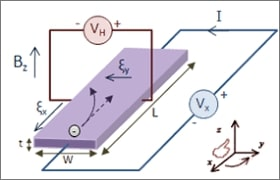
\includegraphics[scale=0.45]{ME20B004.jpg}
	\end{center}}
	\caption{Hall Effect \cite{pic}}
	\label{f1:image}
\end{figure}

Webpage Links \cite{weblink}



\bibliography{bibliography.bib}
